\section{Introduction}
\label{sec:intro}


\subsection{Quantum Computers}
\label{sec:QC}
While quantum computers can be used for analog computation or simulating quantum systems\cite{henrietQuantumComputingNeutral2020}, 
it is also possible to make them perform quantum information processing (QIP). The carriers of information in QIP are qubits. These differ from classical qubits
in that they make use of quantum superposition. Thus a qubit's state (either $|1 \rangle$ or $|0 \rangle$) will remain in superposition until measurement. Prior to this,
the qubit is said to be in a superposition of both states, where the probability of measuring either one of those states is P($|1 \rangle$) + P($|0 \rangle$) = 1\cite{wongIntroductionClassicalQuantum2022a}.
Mathematicaly a qubit is represented as:\\
$ |a \rangle = \alpha|1 \rangle + \beta|0 \rangle =  \begin{bmatrix}
    \alpha \\
    \beta \\
\end{bmatrix}$, where $|\alpha|^2 + |\beta|^2 = P(|1 \rangle) + P(|0 \rangle) = 1$

\begin{wrapfigure}{r}{75mm}
  \centering
  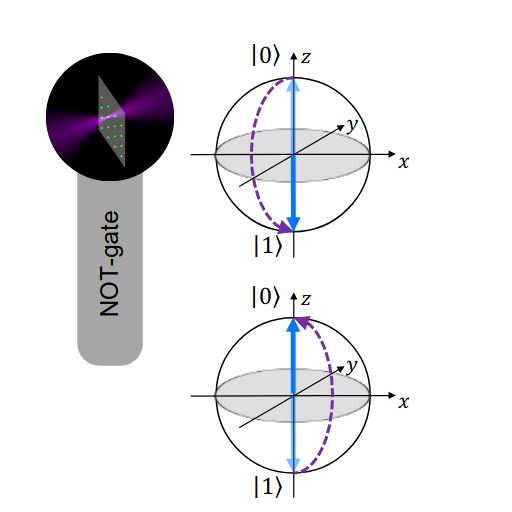
\includegraphics[width=75mm]{./Images/BlochNotGate.png}
  \caption{Bloch sphere representation of the effect of a not (or Pauli $x$) gate. \cite{henrietQuantumComputingNeutral2020}} 
  \label{fig:BlockNotGate}

\end{wrapfigure}


A method to view the state of a qubit before measuring is the Bloch sphere. 
In this representation, the  $|0 \rangle$ state and $|1 \rangle$ state are set to the north and south poles of the sphere respectively\cite{wisemanInterpretationQuantumJump1993}. In addition to the 
probability of getting either state upon measurement, the Bloch sphere shows the phase of the qubit due to the latitudinal direction of the arrow in the sphere\cite{mckayEfficientGatesQuantum2017}.

Before qubit measurement, one can change the state of a qubit using quantum logic gates, which are the quantum computing equivalents of logic 
gates that make up classical electronic circuits. When applied to a qubit, a quantum gate will set it to a specific superposition of states. This corresponds to a 
specific rotation of the arrow on the Bloch sphere\cite{mummaneniLaserControlledImplementationControlledNOT2022}. Since most gates correspond to a rotation and do not place the qubit directly in a specific state, the resulting superposition
depends both on the gate and the state of the qubit before the gate was applied. Some well-known quantum gates are the Pauli $x$ $y$ and $z$ gates, each corresponding to a 
rotation of 180 degrees around the $x$, $y$ and $z$ axes of the Bloch sphere. Gates are mathematically represented as matrices that can be applied to the qubit state vector.
The Pauli $x$ gate for example would be $\begin{bmatrix}
    0 & 1\\
    1 & 0\\
\end{bmatrix}$.

\newpage
Quantum gates are applied to single or multiple qubits at the same time, and in general, these are control gates, which will only affect the target qubit if the control qubit
is already in state $|1 \rangle$. While there are multiple different types of gates, it is possible to create a universal set. Gates in this set can be
combined to create any other gate. The set of arbitrary rotation gates $R_x(\theta), R_y(\theta), R_z(\theta)$, combined with a phase shift gate $P(\varphi)$ and a control-X 
gate are such a set\cite{williamsQuantumGates2011}.


\begin{wrapfigure}{l}{100mm}
  \centering
  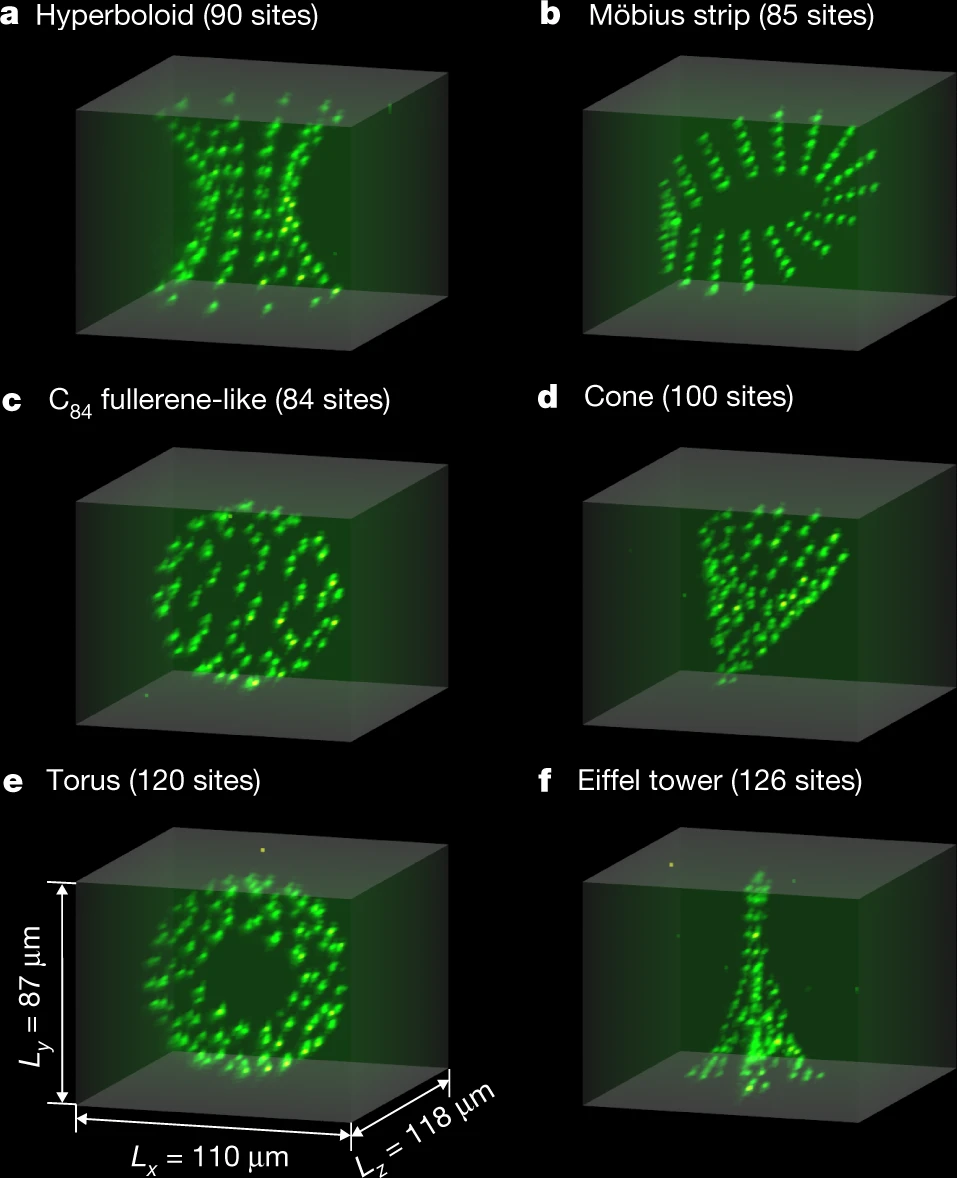
\includegraphics[width=100mm]{./Images/register3D.png}
  \caption{Different qubit configurations in a 3D neutral atom register. \cite{barredoSyntheticThreedimensionalAtomic2018}} 
  \label{fig:3d register}

\end{wrapfigure}
Finally, these qubits are stored in a register. Depending on the type of quantum computer the registry can be fixed, such as for superconducting qubits, where all the qubits 
are pre-engraved onto a chip and used as needed\cite{laddQuantumComputers2010}. Other quantum computers such as the Neutral atom quantum computer built by Pasqal, have a dynamic registry, where a chosen
number of qubits can be placed, at the user's will, into a 2D or 3D grid. This extends the ability of the device to be able to perform simulations of quantum systems and analog
computations that cannot be represented in a traditional quantum circuit.
\\ \\ \\ \\ \\ \\ \\ \\ \\\\

\subsection{QASM}
\label{sec:Qasm}
OpenQASM (Open Quantum Assembly Language) is a programming language for quantum circuits that allows the user to create a register of qubits and comes with a preselection of gates, as well as the universal set of arbitrary rotation,
 phase shift and CX gate. OpenQASM has become the standard for programming quantum circuits, in part due to it being machine-independent, meaning it can be compiled into any
  quantum computer\cite{crossOpenQASMBroaderDeeper2022}. 
  Along with the preset gates, custom user-created gates can be defined and saved to the circuit before compilation and execution. 
  OpenQASM 3 also incorporates timing statements as well as classical computing interactions within a circuit, allowing the user to precisely define when gates or 
  measurements need to be applied, but also allowing the quantum circuit to perform classical operations and interact with a regular processor during the execution of the circuit\cite{crossOpenQASMBroaderDeeper2022}.

  \subsubsection{stdgates.inc}
  stdgates.inc is the file that one can include at the beginning of their QASM code in order to load the preset gates (these can be found in the annex). All the preset gates in this file
 are defined based on a single built-in gate: \\
 the unitary gate $U(\theta,\phi,\lambda) = \begin{bmatrix}
  cos(\theta/2) & -e^{i\lambda}sin(\theta/2)\\
  -e^{i\phi}sin(\theta/2) & -e^{i(\phi+\lambda)}cos(\theta/2)\\
\end{bmatrix} = e^{\phi+\lambda}Rz(\lambda)Rx(\theta)Rz(\phi)$\cite{crossOpenQASMBroaderDeeper2022}\\ \\ 
This gate is combined with modifiers to allow the creation of multi-qubit gates the global phase $gphase(\gamma)$ which adds a global phase of $e^{i\gamma}$ to an operation.
The $ctrl$ and $negctrl$ modifiers are used to test the value of a control qubit before applying the gate which is being modified,
in the case of $ctrl$ the control qubit needs a value of 1 for the operation to proceed and 0 in the case of $negctrl$.
The $inv$ modifier is used to create the inverse $g^{\dagger}$ of a gate $g$ and finally, the $pow(r)$ modifier raises a gate $g$ to the power $g^r$.\cite{crossOpenQASMBroaderDeeper2022}


\subsection{Pasqal's Neutral Atom Quantum Computer}
\label{sec:NAQC}
\subsubsection{Register}
This device uses optical beams to create multiple \SI{1}{\micro\meter\cubed} sized traps\cite{schlosserSubpoissonianLoadingSingle2001}.
Due to their size, these traps can only contain a single atom. The optical beams are then pointed at a vacuum chamber containing atomic vapor and used to single out and reposition atoms into a grid.
\begin{figure}[h]
  \centering
  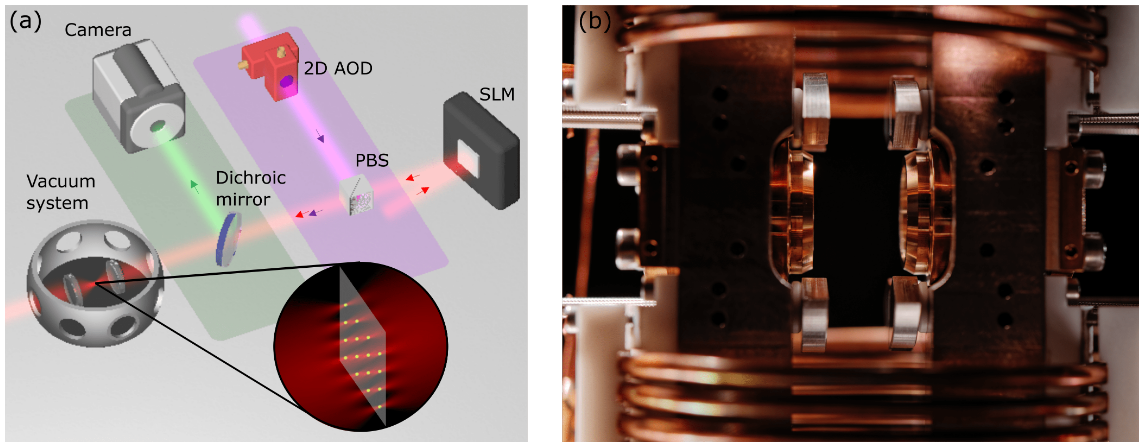
\includegraphics[width=170mm]{./Images/registerHardware.png}
  \caption{"(a) Overview of the main hardware components constituting a quantum processor. The trapping laser light (in red) is shaped by the spatial light modulator (SLM) to produce multiple microtraps at the focal plane of the lens (see inset). The moving tweezers (in purple), dedicated to rearranging the atoms in the register, are controlled by a 2D acousto-optic laser beam deflector (AOD) and superimposed on the main trapping beam with a polarizing beam-splitter (PBS). The fluorescence light (in green) emitted by the atoms is split from the trapping laser light by a dichroic mirror and collected onto a camera. (b) Photography of the heart of a neutral-atom quantum co-processor. The register is prepared at the center of this setup".\cite{henrietQuantumComputingNeutral2020}} 
  \label{fig:hardwareregister}
\end{figure}
\newpage
\subsubsection{Gates}
\begin{wrapfigure}{l}{90mm}
  \centering
  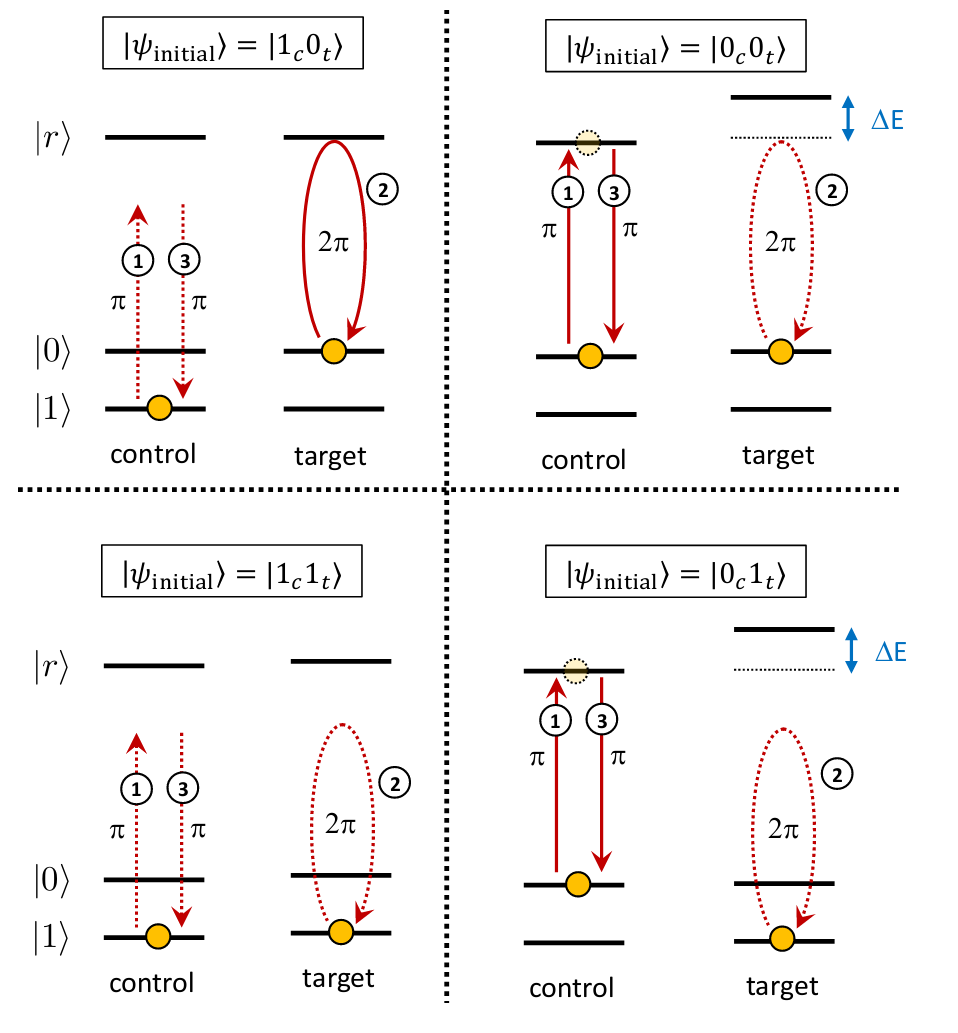
\includegraphics[width=90mm]{./Images/CZbeams.png}
  \caption{Sequence of optical pulses needed for a Control Z gate \cite{silverioPulserOpensourcePackage2022}} 
  \label{fig:CZ}

\end{wrapfigure}
Gates are applied using optical pulses from two different channels: the Raman and Rydberg channels, which can target a single qubit (local) or all of them (global). 
These pulses are used to attain two different excitation states from the ground state $|g \rangle \equiv|0 \rangle$. The Raman pulses are used in single qubit gates to access the hyperfine state $|h \rangle \equiv |1 \rangle$ \cite{tsaiPulselevelSchedulingQuantum2022}.
Multi-qubit gates on the other hand require the use of quantum coherence, which is achieved using a phenomenon called the Rydberg blockade: If an atom is excited to the Rydberg state $|r \rangle$\cite{cohenQuantumComputingCircular2021}(using the Rydberg channel of the quantum device), any nearby atom situated
within a certain radius will be blocked from achieving the Rydberg state \cite{saffmanQuantumComputingAtomic2016}. This interaction is used, for example in the implementation of a CZ gate \cite{saffmanQuantumInformationRydberg2010}. 
\\ \\

\subsubsection{Pulser}

Pasqal has published a Python library named Pulser that simulates their quantum device. It can create a registry with any kind of pattern as well as the required optical pulses.
The pulses have a configurable waveform with amplitude area $\Omega$, detuning $\delta$, phase shifting $\varphi$ and the duration $\tau$ of the pulse. Manipulating these parameters, it is possible to recreate any single-gate rotation on the
 Bloch sphere with angles :
 $$(\Omega\tau\cos\phi,\Omega\tau\sin\phi,\delta\tau)\cite{henrietQuantumComputingNeutral2020}$$
 
 \subsubsection{Pulser's Unitary gate and virtual phase shifts}
Using the above definition, one can create an optical pulse that corresponds directly to a parameterizable unitary gate.
The optical pulse of area $\theta$, detuning $\delta = 0$ and phase $\phi$ corresponds to the Bloch sphere rotation:
\begin{center}
  $R_{Bloch} = R_z(-\phi)R_x(\theta)Rz(\phi)$.\cite{henrietQuantumComputingNeutral2020}
\end{center}
 While this particular pulse for rotations around the $x$ axis when $\phi = 0$ or is a multiple of $\pi$ and $y$ axis when $\phi$ is a multiple of $\pi/2$.
Rotations around the $z$ axis are impossible and need to be implemented via so-called Virtual Z-gates. Since Z gates affect the phase of a qubit and not the probability to measure 0 or 1, virtual 
gates are achieved by applying a phase shift to all the following $x$ and $y$ gates. In Pulser, this is known as a post-phase shift.
Combining this phase shift and the resonant pulses one can create  the gate:
\begin{center}
  $U(\gamma,\theta,\phi) = R_z(\gamma + \phi)R_{Bloch} =  R_z(\gamma + \phi)R_z(-\phi)R_x(\theta)R_z(\phi)$\cite{henrietQuantumComputingNeutral2020}
\end{center}
This actually corresponds to the unitary gate:
\begin{center}
  $U(\gamma,\theta,\phi) = R_z(\gamma)R_x(\theta)R_z(\phi)$\cite{henrietQuantumComputingNeutral2020}
\end{center}
 
It is important to note that this unitary gate differs from the unitary gate defined by QASM in that the middle rotation is an $R_x$ rotation and there is a difference in the global phase.


\subsection{Aim}
There are currently no QASM compilers specific to neutral atom quantum computers, thus this study aims to determine the feasibility of such a project.
This will be done by first establishing whether the required gates for such a task can be implemented on a physical level. Second, the constraints
specifically imposed on register creation need to be identified. Finally, the work on the compiler will start by starting to parse information 
from some of the main commands of QASM. 